%==================================================================
% Ini adalah bab 3
% Silahkan edit sesuai kebutuhan, baik menambah atau mengurangi \section, \subsection
%==================================================================

\chapter[METODOLOGI PENELITIAN]{\\ METODOLOGI PENELITIAN}

\section{Tahapan Penelitian}
Tahapan yang lakukan dalam penelitian ini dapat dilihat pada \cref{fig:tahapan-penelitian}. Penjelasan tahapan
penelitian akan dibahas pada subbab berikutnya
\begin{figure}[H]
    \centering
    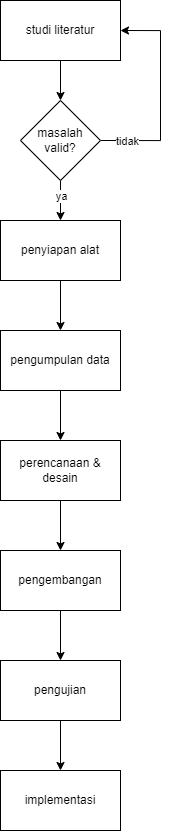
\includegraphics[scale=0.5]{tahapan-penelitian.png}
    \caption{Tahapan Penelitian}
    \label{fig:tahapan-penelitian}
\end{figure}

\subsection{Studi Literatur}
Tahapan pertama yang dilakukan pada penelitian ini adalah dengan melakukan studi literatur. Tahapan studi literatur dilakukan dengan pencarian literatur yang dapat berupa jurnal, paper, buku, dan lain-lain terkait dengan penelitian.

\subsection{Persiapan Alat}
Alat yang akan digunakan ditunjukan pada daftar di bawah. Penggunaan sistem operasi microsoft windows dan GNU linux bertujuan agar dapat memberikan kompatibilitas pada library yang akan dikembangkan dikarenakan umumnya penggunaan sistem operasi microsoft windows dan GNU linux berbasis debian atau ubuntu oleh para peneliti \citep{arora_2020} \citep{stackoverflow}.

\subsubsection{Perangkat Lunak}
\begin{packed_enum}
  \item Python 3
  \item Microsoft Windows 11 22H2
  \item GNU Linux Pop!\_OS 22.04 LTS
  \item Windows Subsystem for Linux (WSL)
\end{packed_enum}

\subsubsection{Perangkat Keras}
\begin{packed_enum}
  \item AMD Athlon Gold 3150U with Radeon Graphics
  \item AMD Radeon Vega 3
  \item 12gb ram DDR4 (10gb usable)
  \item SSD Kingston OM8PCP3512F-AB 512gb (windows)
  \item SSD Adata SU750 1tb (windows)
  \item SSD TeamGroup CX2 256gb via enclosure USB 2.0 (linux)
\end{packed_enum}

\subsection{Pengumpulan Data}
Metode pengumpulan data yang digunakan dalam penelitian ini adalah dengan studi literatur. Studi literatur dilakukan dengan mencari jurnal dan \textit{paper} penelitian terkait tentang algoritma optimasi. Jurnal dan \textit{paper} yang digunakan berkaitan dengan perbandingan, pengembangan, dan \textit{review} algoritma optimasi. Jurnal dan \textit{paper} tersebut menyebutkan fungsi uji yang digunakan dalam penelitian tersebut dan beberapa menuliskan rumus matematika dari fungsi uji yang digunakan dalam penelitian tersebut. Fungsi tersebut umumnya merupakan fungsi uji dari CEC karena kerangka kerja pengujian menggunakan CEC adalah yang paling umum digunakan. Selain dari jurnal dan \textit{paper} digunakan juga sumber dokumentasi resmi dari COCO yang berupa \textit{website} dan file pdf. Penggunaan kerangka kerja pengujian COCO atau \textit{Black-Box Optimization Benchmarking} (BBOB) juga salah satu yang umum digunakan dalam penelitian terkait algoritma optimasi.

\subsection{Perencanaan dan Desain}
Sebelum memulai tahapan pengembangan, perencanaan dan desain \textit{library} dilakukan secara menyeluruh. Proses perencanaan meliputi pembuatan backlog produk yang berisi daftar fitur dan tugas yang harus diselesaikan, estimasi waktu pengerjaan untuk setiap tugas, pembuatan \textit{roadmap} yang menggambarkan alur pengembangan, identifikasi risiko potensial yang dapat menghambat proses, serta penyiapan lingkungan pengembangan yang diperlukan.

Desain \textit{library} mencakup beberapa aspek penting, seperti pendefinisian tujuan dan kebutuhan yang harus dipenuhi oleh \textit{library}, arsitektur dan desain sistem yang akan digunakan, perancangan (\textit{Application Programming Interface}) API yang memungkinkan integrasi dan penggunaan \textit{library} dengan mudah, serta penyusunan rencana dokumentasi yang komprehensif untuk membantu pengguna memahami dan memanfaatkan \textit{library} dengan efektif.

\subsection{Pengembangan}
Proses pengembangan dilakukan dengan menuliskan kode dalam bahasa Python. Tahapan ini mengikuti perencanaan dan desain yang telah disusun sebelumnya. Dalam pengembangan ini, diterapkan paradigma Pemrograman Berorientasi Objek (\textit{Object Oriented Programming} atau OOP) agar \textit{library} yang dikembangkan memiliki arsitektur yang bersih (\textit{clean architecture}) dan terstruktur. Penggunaan OOP bertujuan untuk mempermudah proses pengembangan, pemeliharaan, pengujian, serta awakutu (\textit{debugging}) pada \textit{library}. Dengan pendekatan ini, setiap komponen \textit{library} dapat dikembangkan secara modular, sehingga memudahkan dalam melakukan pengujian unit (\textit{unit testing}) dan mempercepat proses awakutu. \textit{Clean architecture} juga memungkinkan pengembang lain untuk dengan mudah memahami dan mengembangkan lebih lanjut \textit{library} tersebut sesuai kebutuhan.

\subsection{Pengujian}
Pengujian \textit{library} yang dikembangkan dilakukan menggunakan \textit{unit testing}. Pendekatan ini dipilih karena \textit{unit testing} menguji setiap fungsi (unit) secara individu, memastikan bahwa setiap fungsi dalam \textit{library} bekerja dengan baik dan menghasilkan hasil yang konsisten untuk berbagai parameter yang diberikan.

\textit{Unit testing} menawarkan beberapa keuntungan utama. Pertama, pengujian ini memungkinkan hasil yang konsisten karena setiap fungsi diuji secara terpisah dengan parameter yang ditentukan. Kedua, \textit{unit testing} mempermudah dan mempercepat proses pengujian. Dengan hanya perlu memberikan nilai parameter dan nilai hasil yang diharapkan, pengujian dapat dilakukan dengan cepat dan efisien. Selain itu, \textit{unit testing} memungkinkan pengujian berbagai skenario penggunaan dengan mudah. Hal ini dilakukan dengan menduplikasi unit test dan memberikan nilai parameter yang berbeda pada setiap tes, sehingga memastikan bahwa berbagai kondisi dan kasus penggunaan dapat diuji dengan lengkap dan mendetail. Dengan demikian, \textit{unit testing} tidak hanya meningkatkan keandalan dan kualitas \textit{library} yang dikembangkan tetapi juga mempercepat siklus pengembangan perangkat lunak.